\section{Analysis}
\label{sec:analysis}

The analyses below were pre-committed before the grid froze, so the narrative
cannot be retrofitted to the data; each is now populated against the frozen
\resCellsComplete{}-cell grid.

\begin{figure}[t]
  \centering
  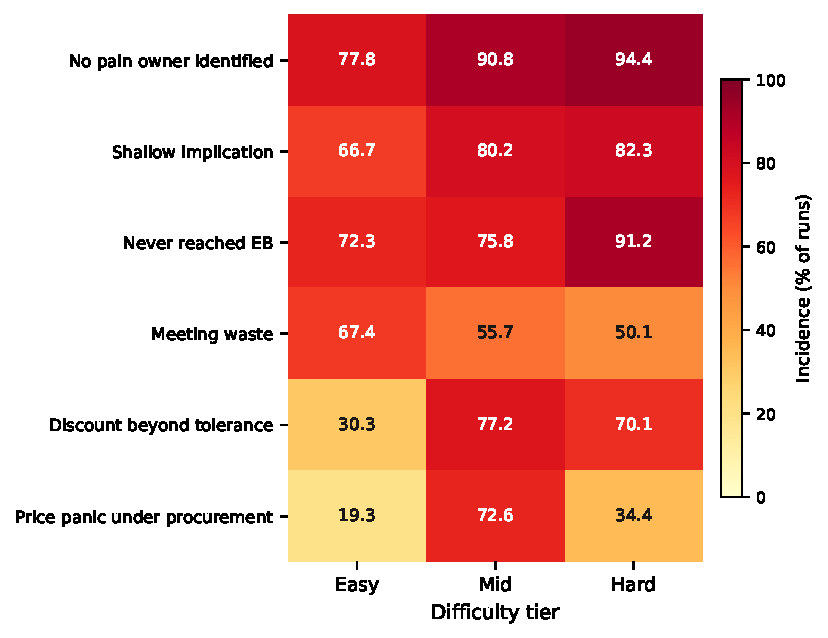
\includegraphics[width=0.7\linewidth]{figures/failure_heatmap.pdf}
  \caption{Failure-mode incidence (percent of runs exhibiting each mode) by
  difficulty tier, pooled over both tracks. Discovery and stakeholder failures
  dominate and worsen monotonically with tier; price failures are near-absent on
  easy deals and spike on the mid tier where the discount-bait events live.}
  \label{fig:failheat}
\end{figure}

\subsection{Where models fail}
Figure~\ref{fig:failheat} reports failure-mode incidence by difficulty tier. The
dominant signatures are diagnostic, not random. The most common failure across the
grid is a discovery failure---\emph{no pain owner identified} (\resFailNoPainOwnerOverall{}\% of runs) and
\emph{shallow implication} (\resFailShallowImplicationOverall{}\%)---and the second is a stakeholder failure,
\emph{never reached the economic buyer} (\resFailNeverEBOverall{}\%). Both worsen monotonically with
tier: never-reached-EB rises $\resFailNeverEBEasy\%\to\resFailNeverEBMid\%\to\resFailNeverEBHard\%$ from easy to hard, and
no-pain-owner rises $\resFailNoPainOwnerEasy\%\to\resFailNoPainOwnerMid\%\to\resFailNoPainOwnerHard\%$. Crucially, the easy tier is not
dominated by capability failures: even on winnable deals, \resFailNeverEBEasy{}\% of runs never reach
the EB and \resFailMeetingWasteEasy{}\% waste a meeting extracting no gated facts---these are
\emph{discipline} failures, exactly the behaviors the methodology pack targets, and
they confirm the hypothesis that easy-tier losses are unforced rather than a ceiling
on model capability. Price failures behave differently: \emph{discount-beyond-tolerance}
and \emph{price-panic-under-procurement} are least common on easy deals
(\resFailDiscountBeyondEasy{}\% and \resFailPricePanicEasy{}\%) but jump to
\resFailDiscountBeyondMid{}\% and \resFailPricePanicMid{}\% on the mid tier, where the discount-bait events live.

\subsection{Does the pack transfer into behavior or only language?}
The central scientific question of the pack track is whether an injected
methodology changes what a model \emph{does} or only what it \emph{says}. The
evidence is that transfer into behavior is real but partial. The pack's SQS lift is
statistically present only where behavioral markers actually move: pooled
EB-attainment rises $\resEBOOB\%\to\resEBPack\%$ and MAP-completion $\resMAPOOB\%\to\resMAPPack\%$, and the
per-tier lift (Table~\ref{tab:lift}) is significant only on the easy tier, where
those behaviors have room to improve. Models that raise EB and MAP rates under the
pack gain SQS; models whose EB/MAP behavior is unchanged gain nothing, even though
all of them adopt the methodology's vocabulary. The pack is therefore a genuine but
bounded intervention: it converts more reliably into process behavior on deals that
are already winnable than into breakthrough on deals gated by access or budget.

\subsection{Difficulty calibration}
The tiers are ordered as designed. Pooled OOB mean SQS decreases monotonically
across tiers ($\resTierSQSEasy\to\resTierSQSMid\to\resTierSQSHard$) as does clean-win
rate ($\resTierCleanEasy\%\to\resTierCleanMid\%\to\resTierCleanHard\%$),
and the failure gradient above corroborates the ordering mechanically rather than by
fiat. No tier ordering inverts at the pooled level, indicating the difficulty axis is
a real gradient and not an artifact of a few idiosyncratic scenarios.

\subsection{Seed variance and matched pairs}
Buyer stochasticity alone is a rich source of preference pairs. Holding model,
scenario, and track fixed and varying only the buyer seed, \resSeedMixedCells{} of
the \resSeedCells{} cells
(\resSeedMixedPct{}\%) contain \emph{both} a clean win and a non-win---episodes identical in
every controllable dimension that diverged only on buyer sampling. The mean
intra-cell SQS standard deviation is \resSeedIntraSD{} points. This is direct evidence that the
seed axis yields the seed-matched win/loss contrasts that preference-based
post-training consumes, and it justifies the chosen seed depth: with fewer seeds a
large fraction of these decisive within-cell disagreements would go unobserved.

\subsection{Cost--capability trade-off}
Figure~\ref{fig:frontier} situates each endpoint on the quality/cost plane.
The result that matters for practitioners is that capability and cost-efficiency do
\emph{not} trade off at the top: the highest-SQS model (\resBestModel{}) is also the
cheapest per closed deal at \$\resCostPerDealMin{}, while the most expensive model
costs \$\resCostPerDealMax{} per deal---a \resCostPerDealSpread$\times$
spread---with no
corresponding quality advantage. The spread survives the change of denominator:
on cost-per-run, which does not divide by (sometimes small) win counts, the same
ordering holds at a $\sim$\resCostPerRunSpread$\times$ spread
(\$\resCostPerRunMin{}--\$\resCostPerRunMax{} per episode), with
\resBestModel{} at \$\resFrontierBestCostPerRun{} per run. The Value Frontier collapses to essentially a
single efficient point, and the expensive Anthropic and reasoning-heavy xAI
endpoints sit strictly inside it: they pay more per token and per deal without
buying better sales outcomes on this task.

\subsection{The reproducible analysis pipeline}
\label{sec:pipeline}
Every number in this paper is produced by a fixed sequence of offline,
deterministic transforms over the persisted transcripts, not by bespoke queries.
We describe it here both for reproducibility and because the pipeline itself
encodes several trust guarantees a reader should be able to check.

\paragraph{One cell, one coordinate.} A graded unit is uniquely a
\texttt{(track, seller, scenario, seed)} coordinate. Because data is collected in
successive batches---and the same coordinate can legitimately reappear across
batches (a re-run, or seeds banked in an earlier canonical release)---the
aggregation step \emph{deduplicates by coordinate before ranking}, keeping a real
LLM-panel grade over any heuristic fallback on collision. This makes pooling all
collection directories idempotent: a coordinate is counted exactly once no matter
how many batches touched it, so the leaderboard cannot be inflated or skewed by
double-counting. The aggregator reports the number of duplicate coordinates it
dropped, so the deduplication is visible rather than silent.

\paragraph{Explicit grid accounting.} The same step reports completion against the
intended rectangular grid---every model $\times$ every scenario $\times$ seeds
$1..\numSeeds{}$ $\times$ both tracks---as a fraction of cells done with the
remainder stated outright. We never report an aggregate without also stating how
much of the grid it rests on, and cells still carrying a heuristic-fallback grade
(Section~\ref{sec:judge}) are counted and surfaced so they can be re-graded before
any result is frozen.

\paragraph{Paired, seeded estimates.} All aggregates carry bootstrap confidence
intervals over seeds, and the headline methodology lift is computed as a
\emph{within-pair} contrast---the same model on the same scenario and seed, pack
versus OOB---via a seeded paired bootstrap, never as a difference of independent
means. A lift is called significant only when its $95\%$ CI excludes zero
\emph{and} rests on at least a minimum number of matched pairs; thinner groups are
flagged as directional rather than reported as fact. The seed is the shared label
that makes the pairing valid (Section~\ref{sec:stochastic}).

\paragraph{Enrichment for open analysis.} Beyond the headline tables, each frozen
grid is expanded into a per-episode feature record---outcome and cost fields, every
scorecard component, price-integrity and discount, and detected failure modes---
emitted as both line-delimited JSON and a flat CSV with an auto-generated data
dictionary. This is what makes the analyses above (failure heatmaps, the
language-versus-behavior gap, difficulty calibration, the cost frontier)
reproducible from a single released artifact, and it is what we invite external
readers to re-analyze. Every stage is covered by unit tests over small fixtures so
that the transforms themselves, not just their outputs, are auditable.
